\documentclass[12pt, a4paper, oneside]{ctexart}
\usepackage{amsmath, amsthm, amssymb, bm, color, graphicx, geometry, mathrsfs,extarrows, braket, booktabs, array, xcolor, fontspec, appendix, float, subfigure, wrapfig, enumitem}
\usepackage[colorlinks,linkcolor=red,anchorcolor=blue,citecolor=blue,urlcolor=blue,menucolor=black]{hyperref}

%%%% 设置中文字体 %%%%
\setCJKmainfont{方正新书宋_GBK.ttf}[BoldFont = 方正小标宋_GBK, ItalicFont = 方正楷体_GBK, BoldItalicFont = 方正粗楷简体]
%%%% 设置英文字体 %%%%
\setmainfont{Times New Roman}
\setsansfont{Calibri}
\setmonofont{Consolas}

%%%% 设置代码块 %%%%
% 在vscode中使用minted需要先配置python解释器, Ctrl+Shift+P, 输入Python: Select Interpreter选择安装了Pygments的Python版本. 再在setting.json中xelatex和pdflatex的参数中加入 "--shell-escape", 即可
% TeXworks中配置方法参考: https://blog.csdn.net/RobertChenGuangzhi/article/details/108140093
\usepackage{minted}
\renewcommand{\theFancyVerbLine}{
    \sffamily\textcolor[rgb]{0.5,0.5,0.5}{\scriptsize\arabic{FancyVerbLine}}} % 修改代码前序号大小
% 加入不同语言的代码块
\newmintinline{cpp}{fontsize=\small, linenos, breaklines, frame=lines}
\newminted{cpp}{fontsize=\small, linenos, breaklines, frame=lines}
\newmintedfile{cpp}{fontsize=\small, linenos, breaklines, frame=lines}
\newmintinline{matlab}{fontsize=\small, linenos, breaklines, frame=lines}
\newminted{matlab}{fontsize=\small, mathescape, linenos, breaklines, frame=lines}
\newmintedfile{matlab}{fontsize=\small, linenos, breaklines, frame=lines}
\newmintinline{python}{fontsize=\small, linenos, breaklines, frame=lines, python3}  % 使用\pythoninline{代码}
\newminted{python}{fontsize=\small, linenos, breaklines, frame=lines, python3}  % 使用\begin{pythoncode}代码\end{pythoncode}
\newmintedfile{python}{fontsize=\small, linenos, breaklines, frame=lines, python3}  % 使用\pythonfile{代码地址}

%%%% 设置行间距与页边距 %%%%
\linespread{1.2}
\geometry{left=2.5cm, right=2.5cm, top=2.5cm, bottom=2.5cm}

%%%% 定理类环境的定义 %%%%
\newtheorem{example}{例}            % 整体编号
\newtheorem{theorem}{定理}[section] % 定理按section编号
\newtheorem{definition}{定义}
\newtheorem{axiom}{公理}
\newtheorem{property}{性质}
\newtheorem{proposition}{命题}
\newtheorem{lemma}{引理}
\newtheorem{corollary}{推论}
\newtheorem{condition}{条件}
\newtheorem{conclusion}{结论}
\newtheorem{assumption}{假设}
\numberwithin{equation}{section}  % 公式按section编号 (公式右端的小括号)
\newtheorem{algorithm}{算法}

\newsavebox{\nameinfo}
\newenvironment{myTitle}[1]{
    \begin{center}
    {\zihao{-2}\bf #1\\}
    \zihao{-4}\it
}{\end{center}}  % \begin{myTitle}{标题内容}作者信息\end{myTitle}
\newcounter{problem}  % 问题序号计数器
\newenvironment{problem}[1][]{\stepcounter{problem}\par\noindent\textbf{题目\arabic{problem}. #1}}{\smallskip\par}
\newenvironment{solution}[1][]{\par\noindent\textbf{#1解答. }}{\smallskip\par}  % 可带一个参数表示题号\begin{solution}{题号}
\newenvironment{note}{\par\noindent\textbf{注记. }}{\smallskip\par}
\newenvironment{remark}{\begin{enumerate}[label=\textbf{注\arabic*.}]}{\end{enumerate}}

%%%% 图片相对路径 %%%%
\graphicspath{{figure/}} % 当前目录下的figure文件夹, {../figure/}则是父目录的figure文件夹
\setlength{\abovecaptionskip}{-0.2cm}  % 缩紧图片标题与图片之间的距离
\setlength{\belowcaptionskip}{0pt} 

%%%% 缩小item,enumerate,description两行间间距 %%%%
\setenumerate[1]{itemsep=0pt,partopsep=0pt,parsep=\parskip,topsep=5pt}
\setitemize[1]{itemsep=0pt,partopsep=0pt,parsep=\parskip,topsep=5pt}
\setdescription{itemsep=0pt,partopsep=0pt,parsep=\parskip,topsep=5pt}

\everymath{\displaystyle} % 默认全部行间公式, 想要变回行内公式使用\textstyle
\DeclareMathOperator*\uplim{\overline{lim}}     % 定义上极限 \uplim_{}
\DeclareMathOperator*\lowlim{\underline{lim}}   % 定义下极限 \lowlim_{}
\DeclareMathOperator*{\argmax}{arg\,max}  % 定义取最大值的参数 \argmax_{}
\DeclareMathOperator*{\argmin}{arg\,min}  % 定义取最小值的参数 \argmin_{}
\let\leq=\leqslant % 简写小于等于\leq (将全部leq变为leqslant)
\let\geq=\geqslant % 简写大于等于\geq (将全部geq变为geqslant)
\DeclareRobustCommand{\rchi}{{\mathpalette\irchi\relax}}
\newcommand{\irchi}[2]{\raisebox{\depth}{$#1\chi$}} % 使用\rchi将\chi居中

%%%% 一些宏定义 %%%%
\def\bd{\boldsymbol}        % 加粗(向量) boldsymbol
\def\disp{\displaystyle}    % 使用行间公式 displaystyle(默认)
\def\tsty{\textstyle}       % 使用行内公式 textstyle
\def\sign{\text{sign}}      % sign function
\def\wtd{\widetilde}        % 宽波浪线 widetilde
\def\R{\mathbb{R}}          % Real number
\def\N{\mathbb{N}}          % Natural number
\def\Z{\mathbb{Z}}          % Integer number
\def\Q{\mathbb{Q}}          % Rational number
\def\C{\mathbb{C}}          % Complex number
\def\K{\mathbb{K}}          % Number Field
\def\P{\mathbb{P}}          % Polynomial
\def\N{\mathbb{N}}          % Natural number
\def\Z{\mathbb{Z}}          % Integer number
\def\E{\mathbb{E}}          % Exception
\def\var{\text{Var}}        % Variance
\def\cov{\text{Cov}}        % Coefficient of Variation
\def\bias{\text{bias}}      % bias
\def\d{\mathrm{d}}          % differential operator
\def\e{\mathrm{e}}          % Euler's number
\def\i{\mathrm{i}}          % imaginary number
\def\re{\mathrm{Re}}        % Real part
\def\im{\mathrm{Im}}        % Imaginary part
\def\res{\mathrm{Res}}      % Residue
\def\L{\mathcal{L}}         % Loss function
\def\O{\mathcal{O}}         % 时间复杂度
\def\wdh{\widehat}          % 宽帽子 widehat
\def\ol{\overline}          % 上横线 overline
\def\ul{\underline}         % 下横线 underline
\def\add{\vspace{1ex}}      % 增加行间距
\def\del{\vspace{-1.5ex}}   % 减少行间距

%%%% 正文开始 %%%%
\begin{document}
\begin{myTitle}{CVPR第五次作业-目标检测}
    强基数学\\
    吴天阳\quad 2204210460,马煜璇\quad 2204220461,申宇环\quad 2201422097,\\
    陈开来\quad 2205110920,王瑞恒\quad 2202113454
\end{myTitle}
\section{实验目的}
\begin{enumerate}
  \item 掌握HOG特征描述子和线性SVM分类算法.
  \item 理解滑动窗口进行目标检测方法.
  \item 掌握交并比(IoU)的原理与运用.
  \item 理解召回率、检验精度的概念,使用均值平均精度(mAP)评估目标检测器.
\end{enumerate}

具体方法:使用HOG特征和SVM设计单目标检测器.
\section{实验原理}
\subsection{方向梯度直方图(Hog)}
\subsubsection{图像预处理}
对原图像进行高斯模糊,降低噪声,利用Gamma校正公式对原图像亮度进行降低,$f(x) = x^{\gamma},\ (\gamma \geq 1)$,当$\gamma$越大时,图像亮度越低.
\subsubsection{梯度图计算}
使用Sobel算子分别计算$x$和$y$方向的偏导,两个方向上的偏导Sobel算子如下
\begin{equation*}
  W_x = \left[\begin{matrix}
    -1&0&1\\
    -2&0&2\\
    -1&0&1
  \end{matrix}\right],\quad W_y = \left[\begin{matrix}
    -1&-2&-1\\
    0&0&0\\
    1&2&1
  \end{matrix}\right]
\end{equation*}然后计算幅值(L2范数)和梯度方向:
\begin{equation*}
  g = \sqrt{g_x^2+g_y^2},\quad \theta = \left|\arctan\frac{g_y}{g_x}\right|
\end{equation*}
注:此处的梯度方向$\theta$是取过绝对值的结果,所以角度范围为$[0,\pi]$.
\subsubsection{梯度直方图计算}
由于梯度过于离散,对一个较大区域中全部梯度方向进行统计,首先假定cell大小为图像中$8\times 8$的一个区域,将原图划分为多个不交的$8\times 8$的区域,期望将$[0,\pi]$平均划分为$9$个部分(bins),然后将该区域中的梯度均摊到这$9$个辐角区间中来表示这个区域的辐角分布,如下$10$个端点构成的$9$个连续区间
\begin{equation*}
  \pi: 0,20^\circ, 40^\circ, 60^\circ, 80^\circ, 100^\circ, 120^\circ, 140^\circ, 160^\circ, 180^\circ
\end{equation*}
这也就是创建了大小为$9$的直方图数组,记为$h_1,\cdots,h_9$,然后该cell包含的每个像素点处的幅值按该像素点处的方向大小平均分配到最近的区间上即可.

举个例子,如果某像素点的幅值为$4$辐角为$65^\circ$,那么最近的两个区间点为$60^\circ, 80^\circ$对应数组为$h_4,h_5$,并且通过距离确定到两点的权重分别为$1/4,\ 3/4$,于是更新直方图数组为$h_4\rightarrow h_4+1/4\times 4,\ h_5\rightarrow h_5+3/4\times 4$.
\subsubsection{Block归一化}
计算出每个Cell的梯度直方图之后,再以$3\times 3$的cell作为一组,称为block. 由于每个cell包含$9$个值,所以一个block具有$3\times 3\times 9=81$个值,然后在通过滑动步长为$1$的block窗口,逐步输出每个位置的block值,最后拉成一个行向量,这就是\textbf{Hog特征},假设原图的大小为$40\times 100$,则cell个数为$5\times 12$,于是最终Hog特征维数为$(5-3+1)\times(12-3+1)\times 3\times 3\times 9 = 2430$.

再分析下每个block具体做些什么:一个block是由$3\times 3 = 9$个cell构成的,每个cell有$9$个变量,所以一共block存储的是$81$维向量,对齐进行归一化处理,就得到了该block所具有的信息.

\section{实验步骤与结果分析}
本次代码难度较大,参考老师教程使用GitHub中项目完成. 特征提取及SVM模型训练:\href{https://github.com/bikz05/object-detector/tree/master/object-detector}{GitHub-bikz05/object-detector},mAP评价目标检测器:\href{https://github.com/Cartucho/mAP}{Cartucho/mAP}
\subsection{计算Hog特征}
首先利用\pythoninline{extract-features.py}进行Hog特征提取,使用\pythoninline{skimage.feature.hog}对目标进行提取,正例图像处理的核心代码如下(处理反例只需将文件路径修改即可):
\begin{pythoncode}
for im_path in glob.glob(os.path.join(pos_im_path, "*")):  # 读取图片路径
    im = cv2.imread(im_path, cv2.IMREAD_GRAYSCALE)  # 灰度图像读入
    fd = feature.hog(im, orientations=9,  # 将角度分为9个区间
                      pixels_per_cell=(8, 8),  # cell大小
                      cells_per_block=(3, 3))  # block大小
    fd_name = os.path.split(im_path)[1].split(".")[0] + ".feat"
    fd_path = os.path.join(pos_feat_ph, fd_name)  # 设置保存文件路径
    joblib.dump(fd, fd_path)  # 保存图像的Hog特征
\end{pythoncode}

图\ref{fig-hog}是我们自己尝试Hog特征提取结果:
\begin{figure}[htbp]
  \hspace*{-1.2cm}
  \centering
  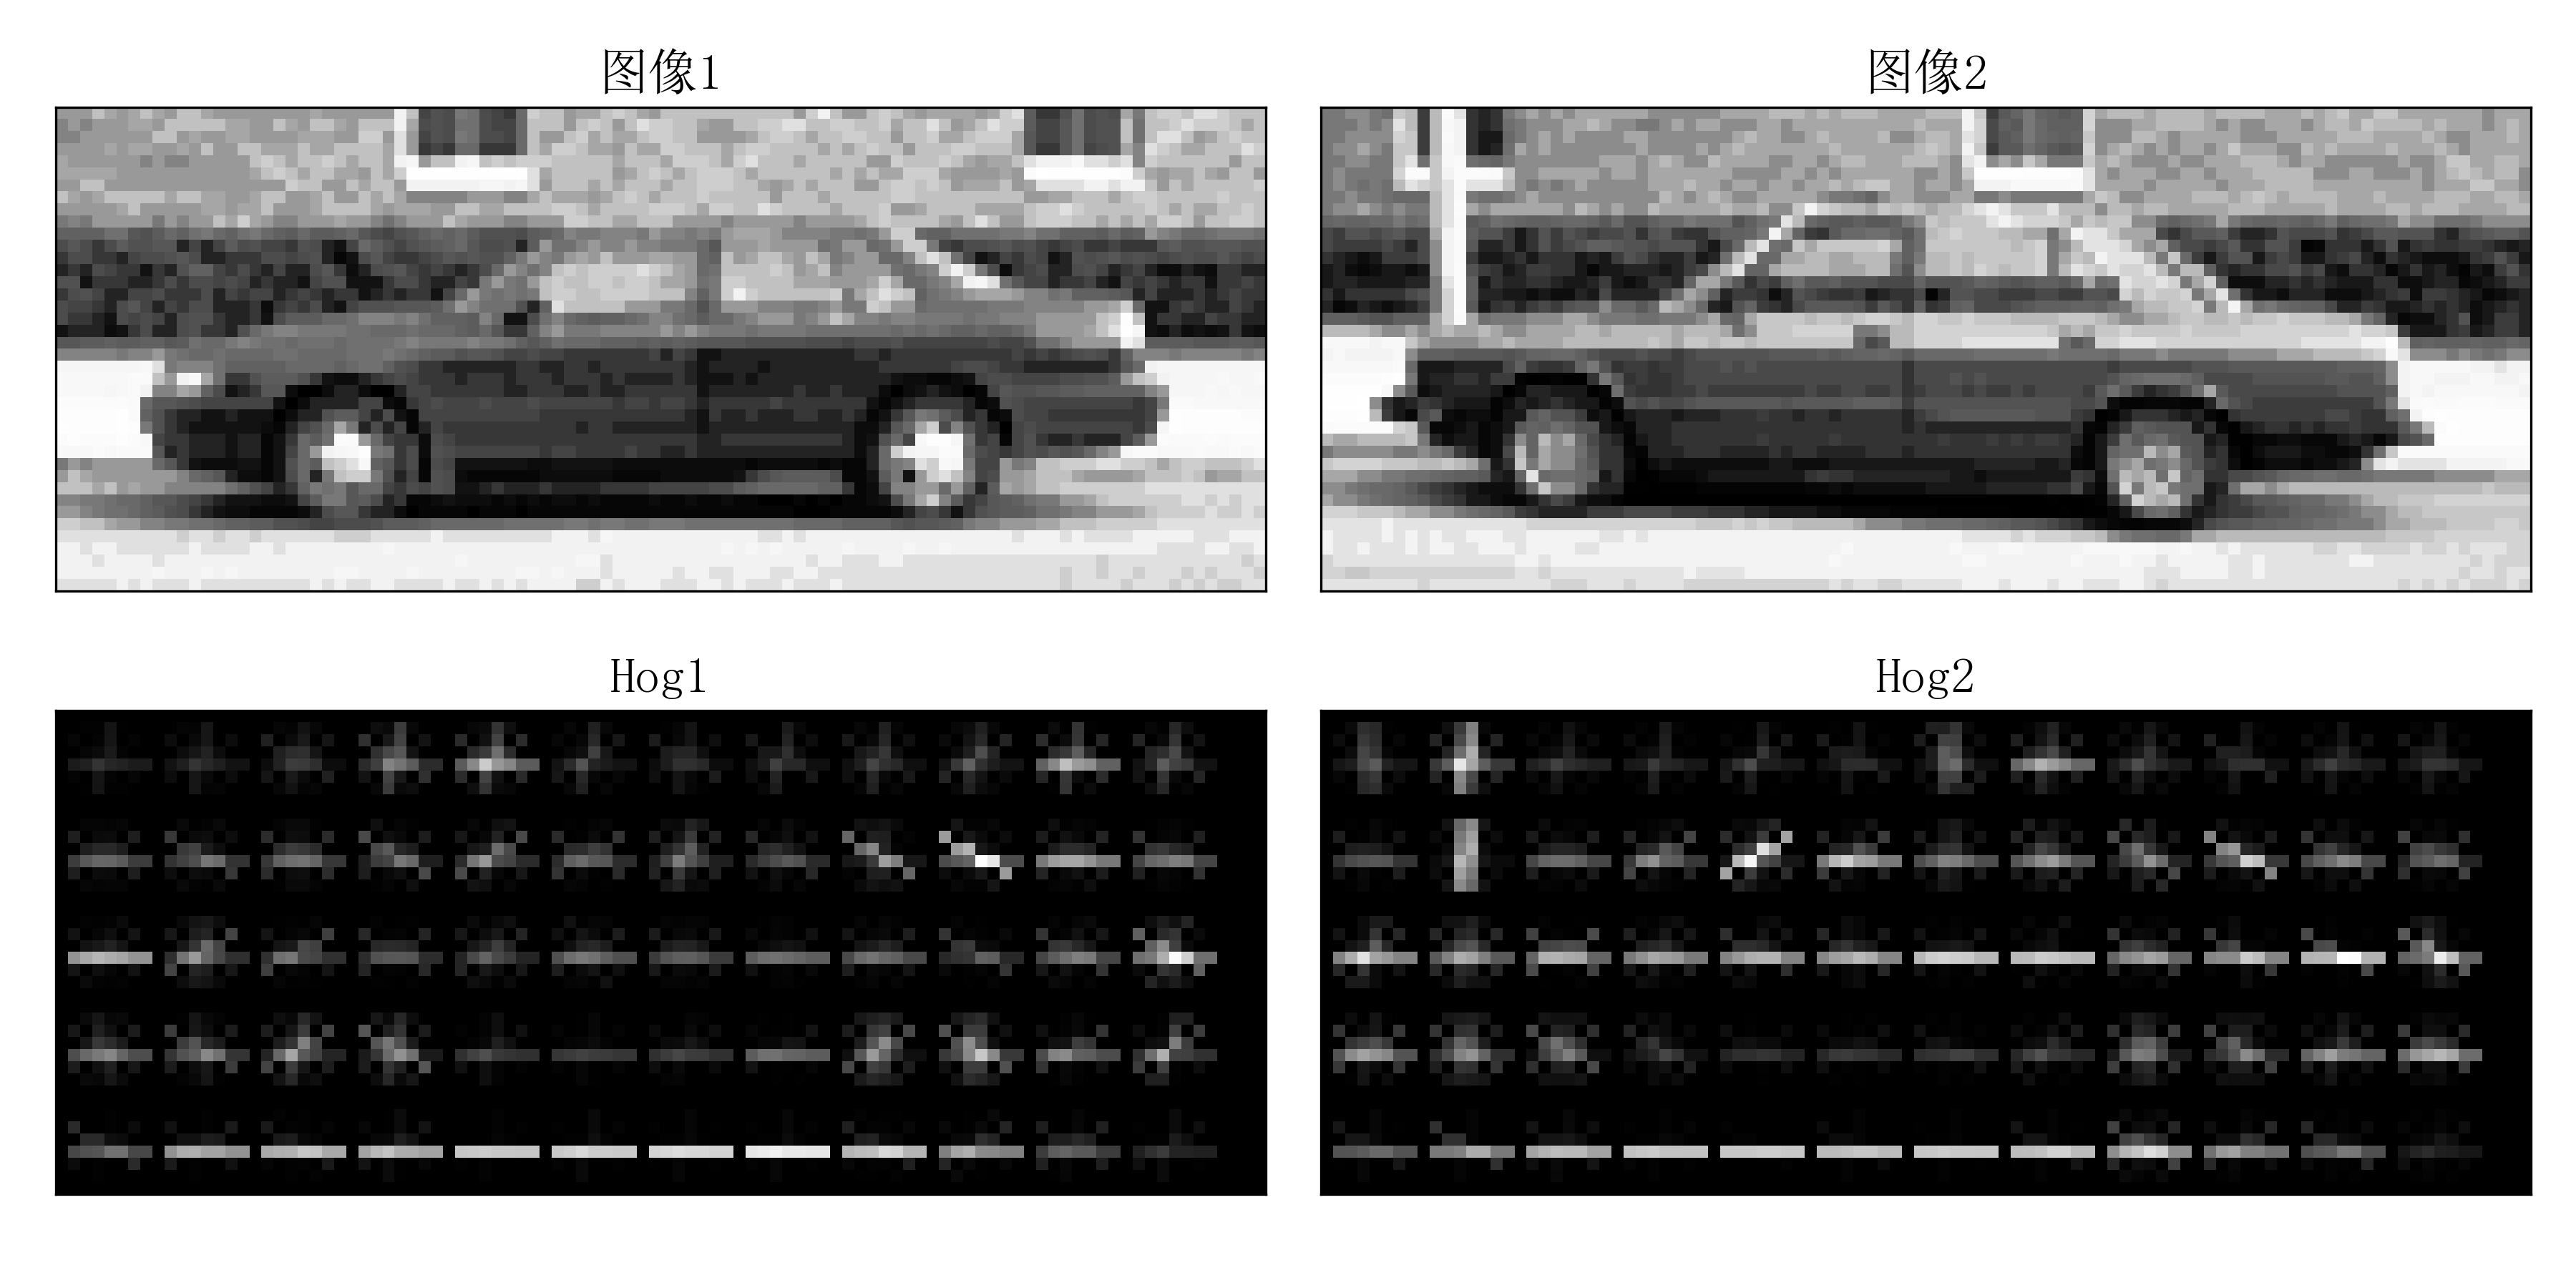
\includegraphics[scale=0.6]{hog特征提取.png}
  \title{Hog特征提取}
  \label{fig-hog}
\end{figure}
\section{结论与讨论}
\end{document}